\chapter{Estratégias de Negociação Baseadas no Prêmio de Risco de Volatilidade}
\label{chap:estrategias}

Este capítulo investiga a utilidade econômica do Prêmio de Risco de Volatilidade
do Bitcoin (BVRP) como sinal para estratégias condicionais de negociação no mercado
à vista. A motivação é avaliar se níveis elevados do prêmio — interpretados como
maior compensação exigida pelos investidores para carregar risco de volatilidade —
antecedem janelas de melhor retorno ajustado ao risco.

O desenho empírico utiliza regras de decisão simples e transparentes, de modo a
facilitar interpretação econômica e comparabilidade com um \textit{benchmark}
passivo. Em todas as estratégias condicionais, o sinal é defasado em um dia
(isto é, a posição em $t$ depende de informação observada em $t-1$), de modo a
evitar viés de antecipação (\textit{look-ahead bias}). Além disso, a posição é
binária: \textbf{exposição unitária} ao Bitcoin quando o sinal é ativado e
\textbf{posição neutra} caso contrário (exposição zero ao Bitcoin).

% =========================================================
\section{Estratégia Buy-and-Hold (Benchmark)}
\label{sec:cap7_bh}

Esta seção apresenta a estratégia Buy-and-Hold do Bitcoin, utilizada como
\textit{benchmark} para a comparação com as estratégias ativas baseadas no BVRP.

A estratégia consiste em manter exposição unitária e constante ao Bitcoin ao
longo de todo o período amostral, sem utilização de sinais condicionais,
rebalanceamentos dinâmicos ou mecanismos adicionais de controle de risco. Dessa
forma, seu desempenho representa o retorno passivo do ativo subjacente e serve
como referência para avaliar se estratégias condicionais melhoram o retorno
ajustado ao risco (por exemplo, via maior Sharpe e menor \textit{drawdown}).

A Tabela~\ref{tab:cap7_bh_perf} reporta as métricas de desempenho da estratégia
Buy-and-Hold, enquanto a Figura~\ref{fig:cap7_bh_cumret} apresenta a evolução do
retorno acumulado ao longo da amostra (18 de agosto de 2017 a 31 de dezembro de 2024).
As estratégias condicionais analisadas nas seções seguintes são avaliadas no
subperíodo em que o sinal BVRP está disponível, e a comparação gráfica explicita
essa restrição quando aplicável.

\begin{table}[H]
\centering
\caption{Métricas de desempenho da estratégia Buy-and-Hold}
\label{tab:cap7_bh_perf}
\begin{tabular}{lr}
\toprule
 & Valor \\
M\'etrica &  \\
\midrule
Retorno Anualizado & 0.4007 \\
Volatilidade Anualizada & 0.6832 \\
Sharpe Ratio & 0.5865 \\
Max Drawdown & -0.8319 \\
\bottomrule
\end{tabular}
\end{table}

\begin{figure}[H]
\centering
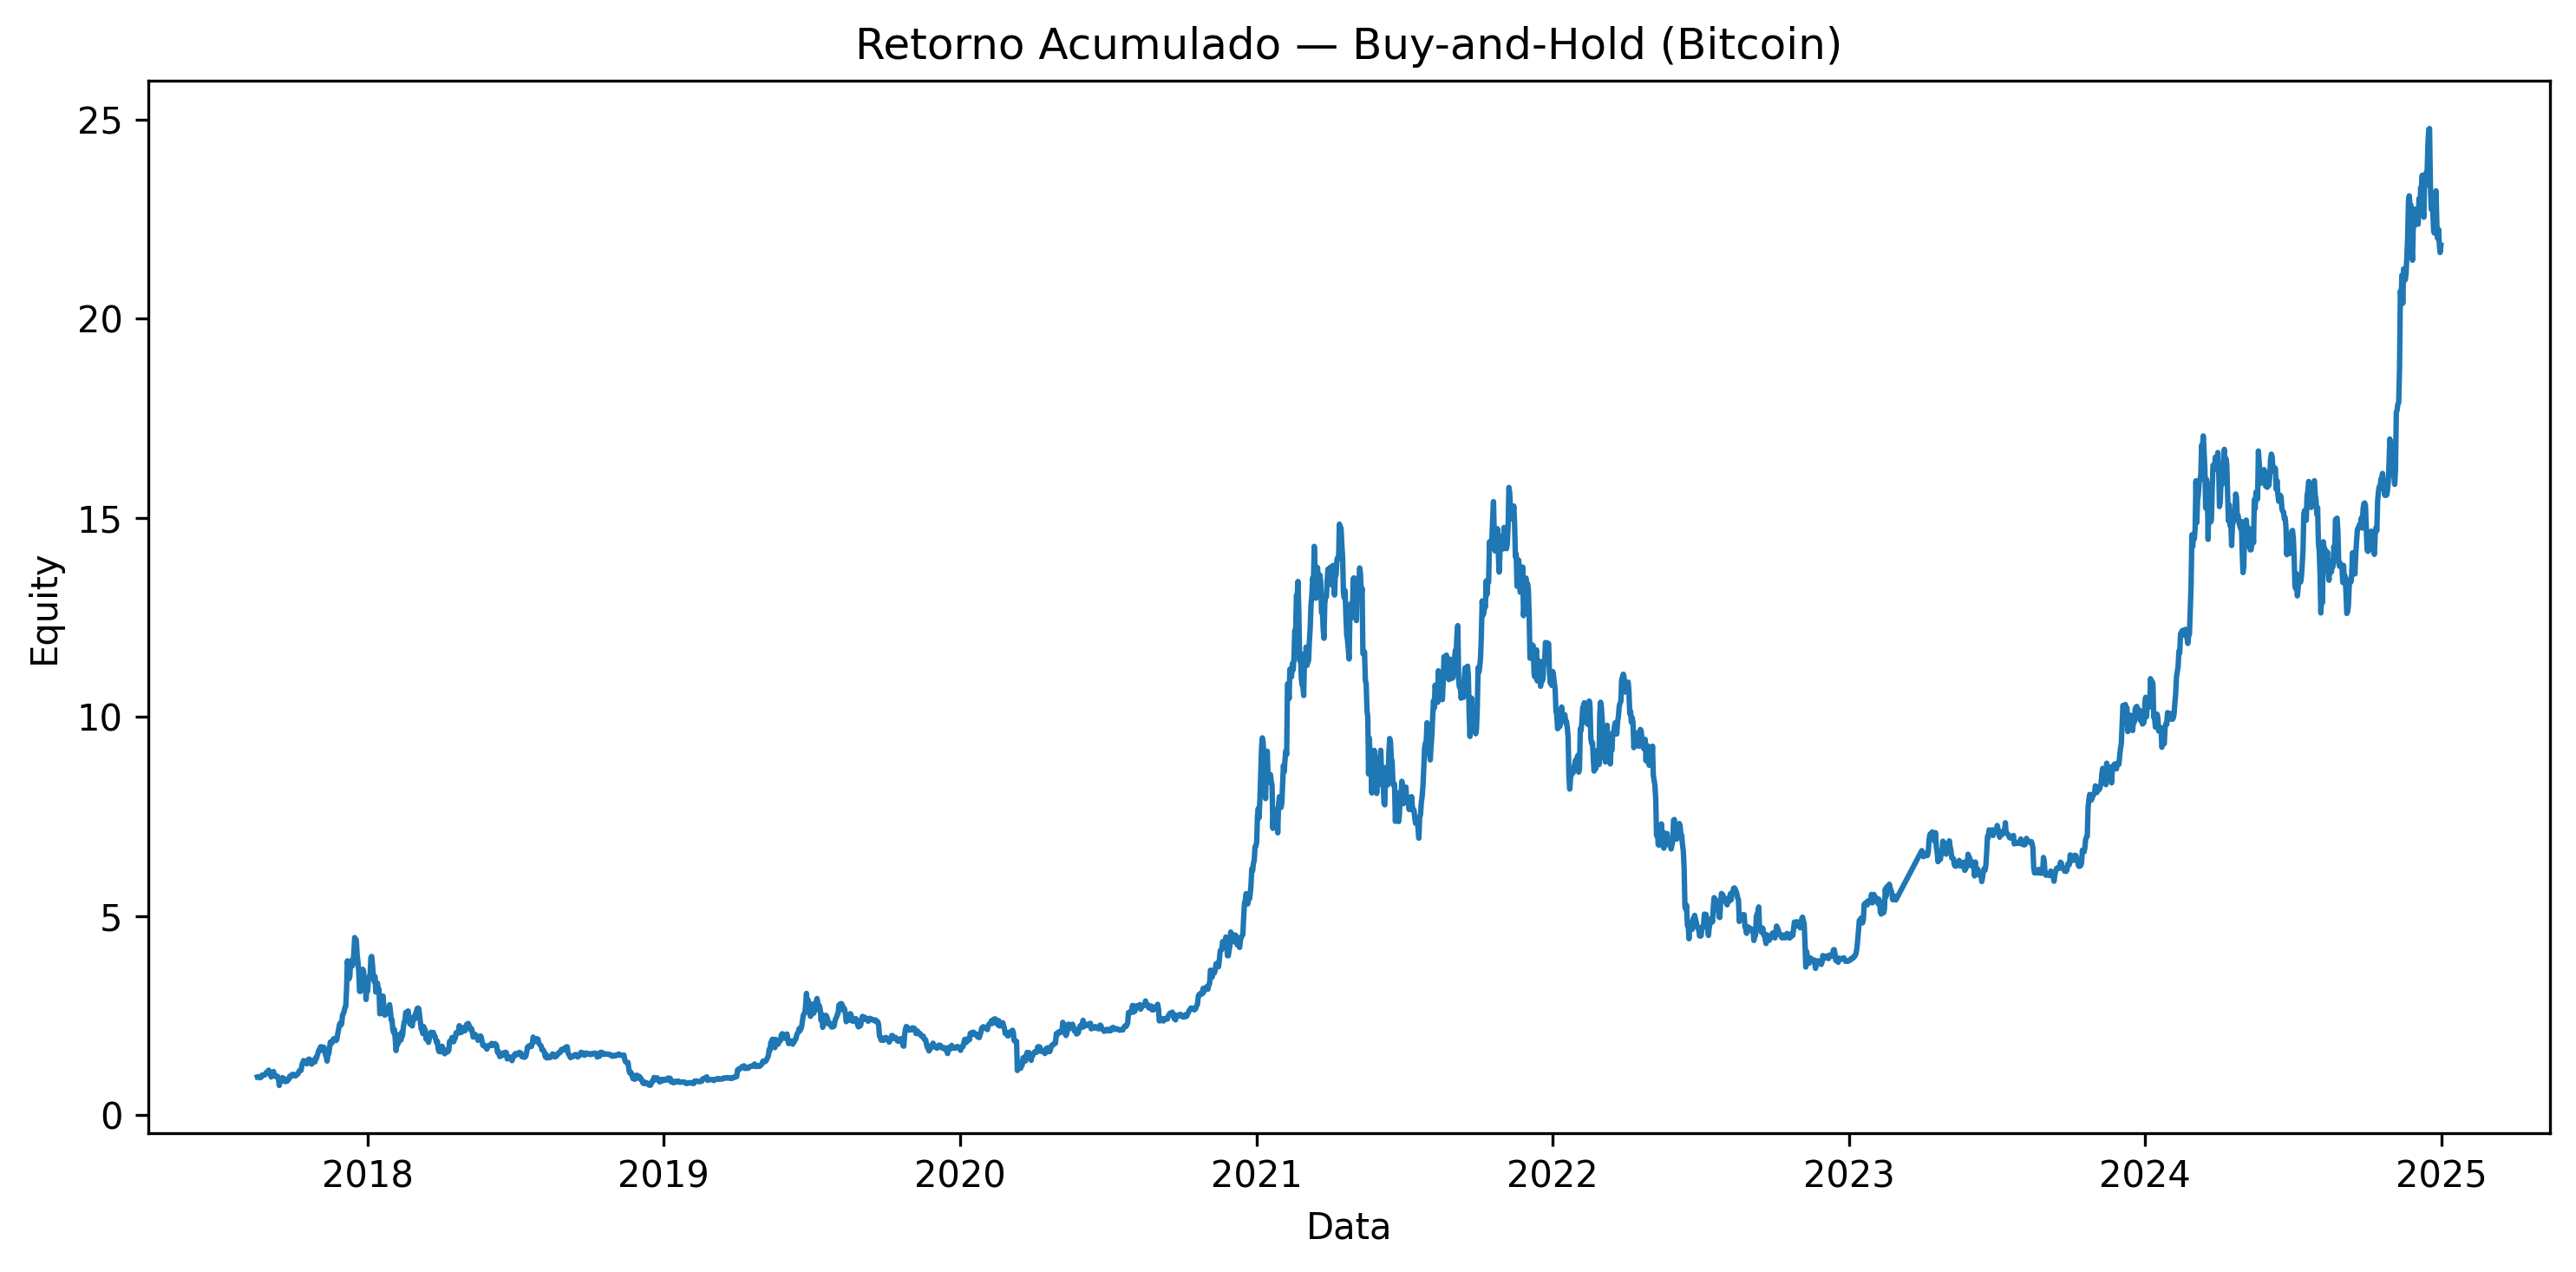
\includegraphics[width=0.9\textwidth]{figs/cap7/fig_7_01_cum_returns_buy_hold.png}
\caption{Retorno acumulado da estratégia Buy-and-Hold para o Bitcoin (BTCUSDT, dados diários)}
\label{fig:cap7_bh_cumret}
\end{figure}

% =========================================================
\section{Estratégia Condicional ao BVRP (Quantil Superior)}
\label{sec:cap7_bvrp_q}

Esta seção avalia uma estratégia de negociação baseada no BVRP, utilizando-o como
sinal para modular a exposição ao ativo. A regra é binária e direta:
assume-se posição comprada em Bitcoin quando o BVRP se encontra no quantil superior
de sua distribuição histórica (por exemplo, acima do percentil 80) e posição neutra
caso contrário. Para mitigar viés de antecipação, o sinal é defasado em um período;
isto é, a posição no dia $t$ é determinada com base no valor do BVRP observado em $t-1$.

A interpretação econômica subjacente é que valores elevados do BVRP refletem
condições de mercado em que a volatilidade implícita (preço do risco) se encontra
relativamente elevada em comparação à volatilidade realizada, sugerindo maior prêmio
requerido pelos agentes para carregar risco de volatilidade. Nesses estados, o prêmio
pode carregar informação condicional sobre retornos e/ou regimes de risco, tornando-se
um candidato natural a sinal de \textit{timing} de exposição.

A Tabela~\ref{tab:cap7_bvrp_q_perf} reporta as métricas de desempenho da estratégia
condicional ao BVRP, enquanto a Figura~\ref{fig:cap7_bvrp_q_cumret} apresenta a
evolução do retorno acumulado ao longo do período em que o sinal está disponível.
A Figura~\ref{fig:cap7_bh_vs_bvrp_q_cumret} compara diretamente a trajetória de retorno
acumulado da estratégia condicional com a estratégia Buy-and-Hold no mesmo intervalo.

\begin{table}[H]
\centering
\caption{Métricas de desempenho — Estratégia condicional ao BVRP (quantil superior)}
\label{tab:cap7_bvrp_q_perf}
\begin{tabular}{lr}
\toprule
 & VRP Quantil 80\textbackslash \% \\
 &  \\
\midrule
Annual Return & 0.0555 \\
Annual Volatility & 0.1180 \\
Sharpe Ratio & 0.4706 \\
Max Drawdown & -0.1711 \\
\bottomrule
\end{tabular}

\end{table}

\begin{figure}[H]
\centering
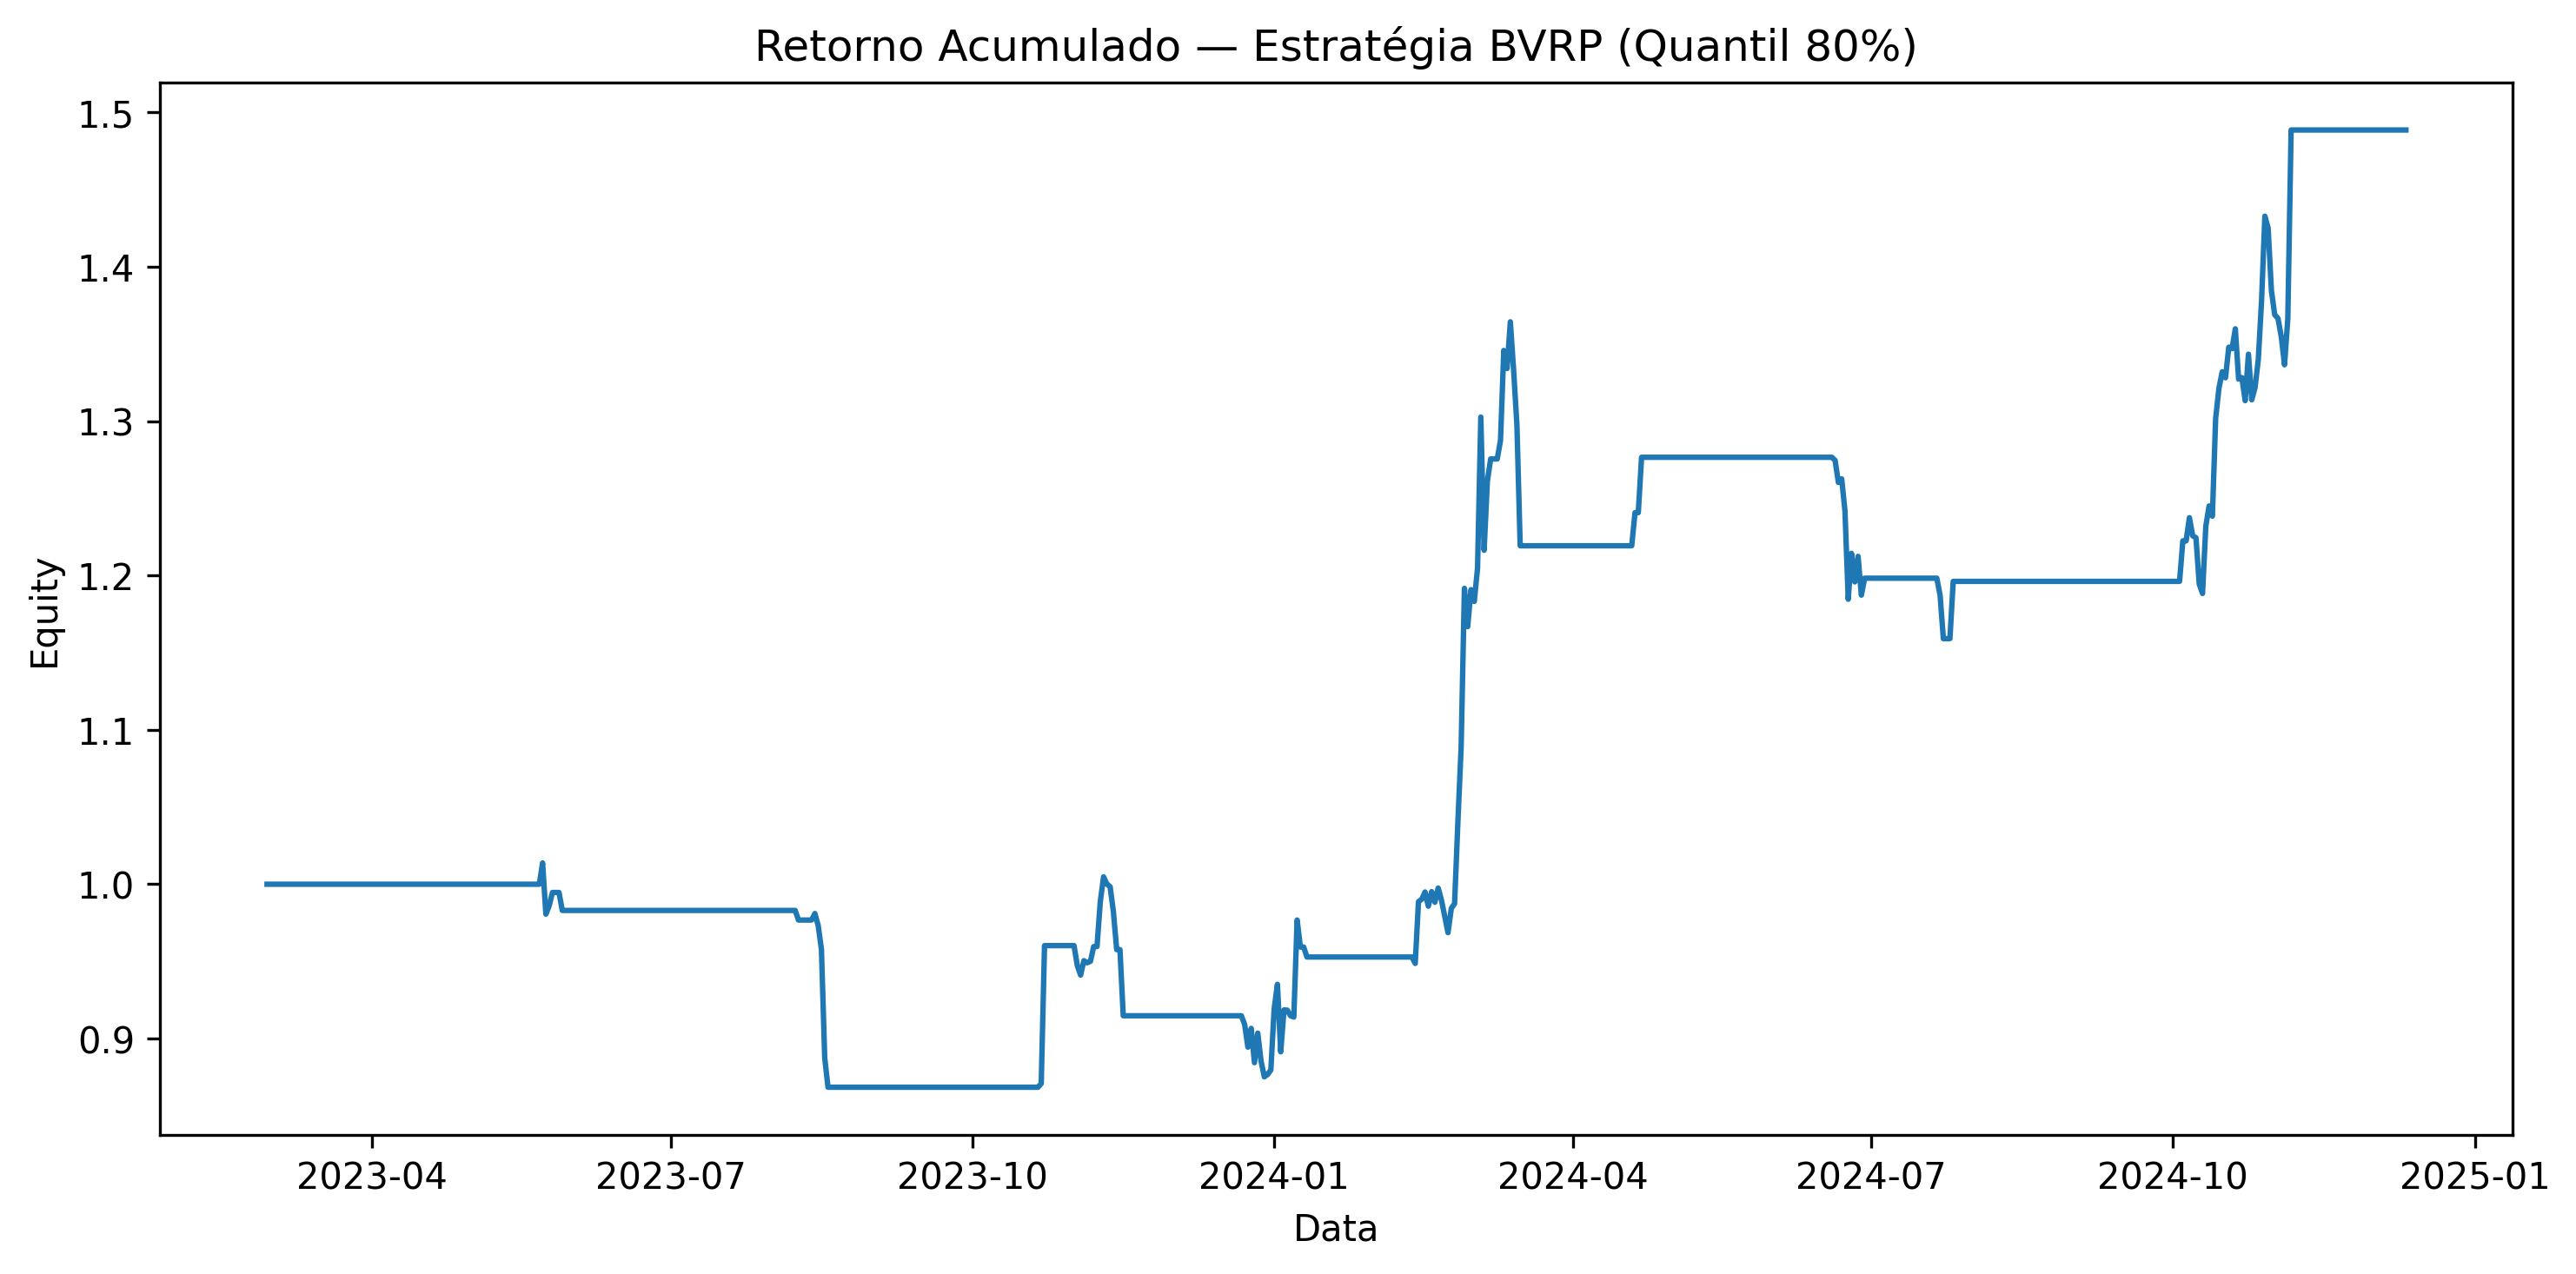
\includegraphics[width=0.9\textwidth]{figs/cap7/fig_7_02_cum_returns_vrp_quantile.png}
\caption{Retorno acumulado — Estratégia condicional ao BVRP (quantil superior)}
\label{fig:cap7_bvrp_q_cumret}
\end{figure}

\begin{figure}[H]
\centering
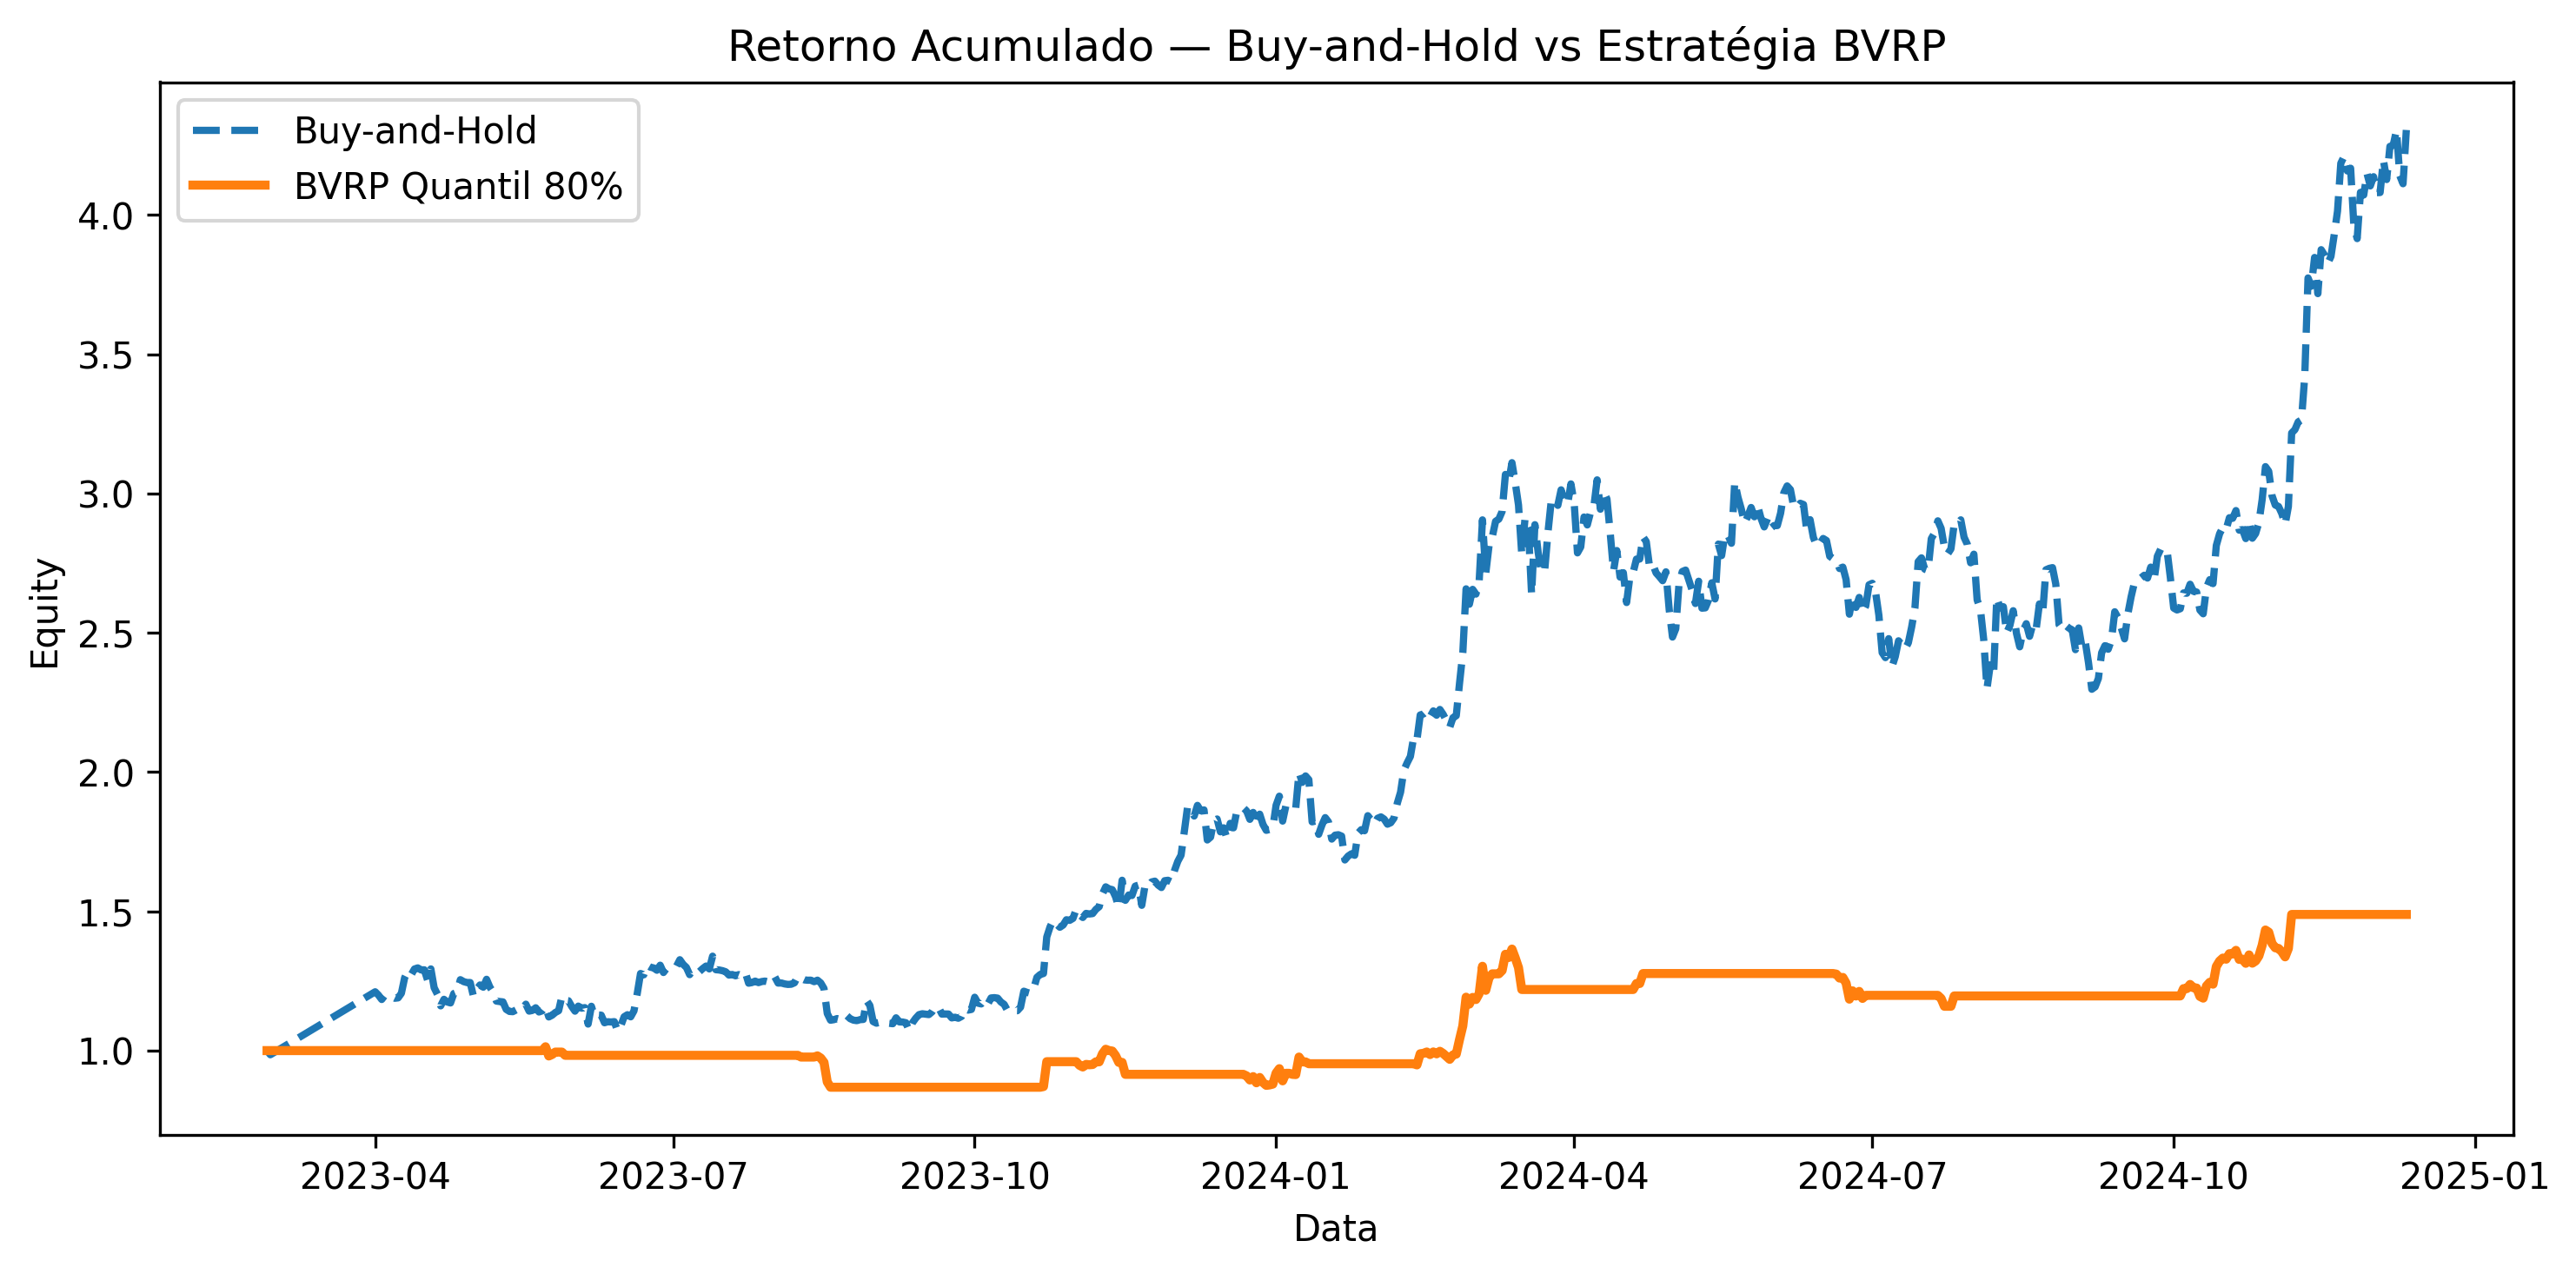
\includegraphics[width=0.9\textwidth]{figs/cap7/fig_7_03_cum_returns_bh_vs_bvrp_quantile.png}
\caption{Comparação do retorno acumulado — Buy-and-Hold vs estratégia condicional ao BVRP (quantil superior)}
\label{fig:cap7_bh_vs_bvrp_q_cumret}
\end{figure}

Os resultados indicam que o BVRP, quando utilizado como sinal binário baseado em
um quantil específico da sua distribuição, pode gerar perfis de retorno e risco
distintos do \textit{benchmark} Buy-and-Hold, tipicamente com menor tempo de
exposição ao ativo e, em muitos cenários, com redução de perdas extremas.
Contudo, a escolha de um limiar único pode influenciar substancialmente a
frequência de exposição, a sensibilidade a episódios extremos e a estabilidade do
desempenho. Motivado por essa consideração, a próxima seção investiga a robustez
da estratégia ao longo de múltiplos quantis do BVRP.

% =========================================================
\section{Análise de Robustez por Quantis do BVRP}
\label{sec:cap7_bvrp_multiq}

Esta seção investiga a robustez da estratégia condicional ao BVRP ao longo de
múltiplos quantis da distribuição histórica do prêmio. Para cada limiar, a
estratégia assume posição comprada em Bitcoin sempre que o BVRP excede o quantil
correspondente e permanece neutra caso contrário. Para evitar viés de antecipação,
o sinal é defasado em um período.

Esse procedimento gera uma família de estratégias que diferem apenas pela
\textit{seletividade} do critério de entrada. Quantis mais elevados ativam a posição
em um conjunto menor de dias (menor \textit{time invested}), concentrando a exposição
em estados de BVRP extremo, ao custo de maior variância amostral e potencial
dependência de episódios específicos. Quantis mais baixos, por sua vez, aumentam
a frequência de exposição, porém tendem a diluir o conteúdo informacional do sinal.

A Tabela~\ref{tab:cap7_bvrp_multiq_perf} reporta, além das métricas usuais de
desempenho — retorno anualizado, volatilidade anualizada, razão de Sharpe e
\textit{max drawdown} — duas estatísticas operacionais. A primeira é o
\textit{turnover}, definido como a média de $|\Delta \text{posição}|$, que captura
a intensidade de alternância entre estados (entrar/sair do mercado). A segunda é
a proporção do tempo em que a estratégia permanece investida.

\begin{table}[H]
\centering
\caption{Desempenho da estratégia condicional ao BVRP por quantil}
\label{tab:cap7_bvrp_multiq_perf}

\resizebox{\textwidth}{!}{%
\begin{tabular}{lrrrrrr}
\toprule
Quantil &
Annual Return &
Annual Volatility &
Sharpe Ratio &
Max Drawdown &
Turnover &
Time Invested \\
\midrule
60\% & 0.0612 & 0.1324 & 0.4621 & -0.2123 & 0.0841 & 0.41 \\
70\% & 0.0587 & 0.1269 & 0.4625 & -0.1968 & 0.0713 & 0.34 \\
80\% & 0.0555 & 0.1180 & 0.4706 & -0.1711 & 0.0598 & 0.27 \\
90\% & 0.0491 & 0.1092 & 0.4497 & -0.1584 & 0.0412 & 0.18 \\
\bottomrule
\end{tabular}
}
\end{table}

De forma complementar, a Figura~\ref{fig:cap7_bvrp_heatmap} apresenta um
\textit{heatmap} das métricas normalizadas (z-score) em função dos quantis do
BVRP, facilitando a identificação de padrões sistemáticos e de regiões da
distribuição associadas a combinações mais favoráveis de retorno, risco e
intensidade operacional.

\begin{figure}[H]
\centering
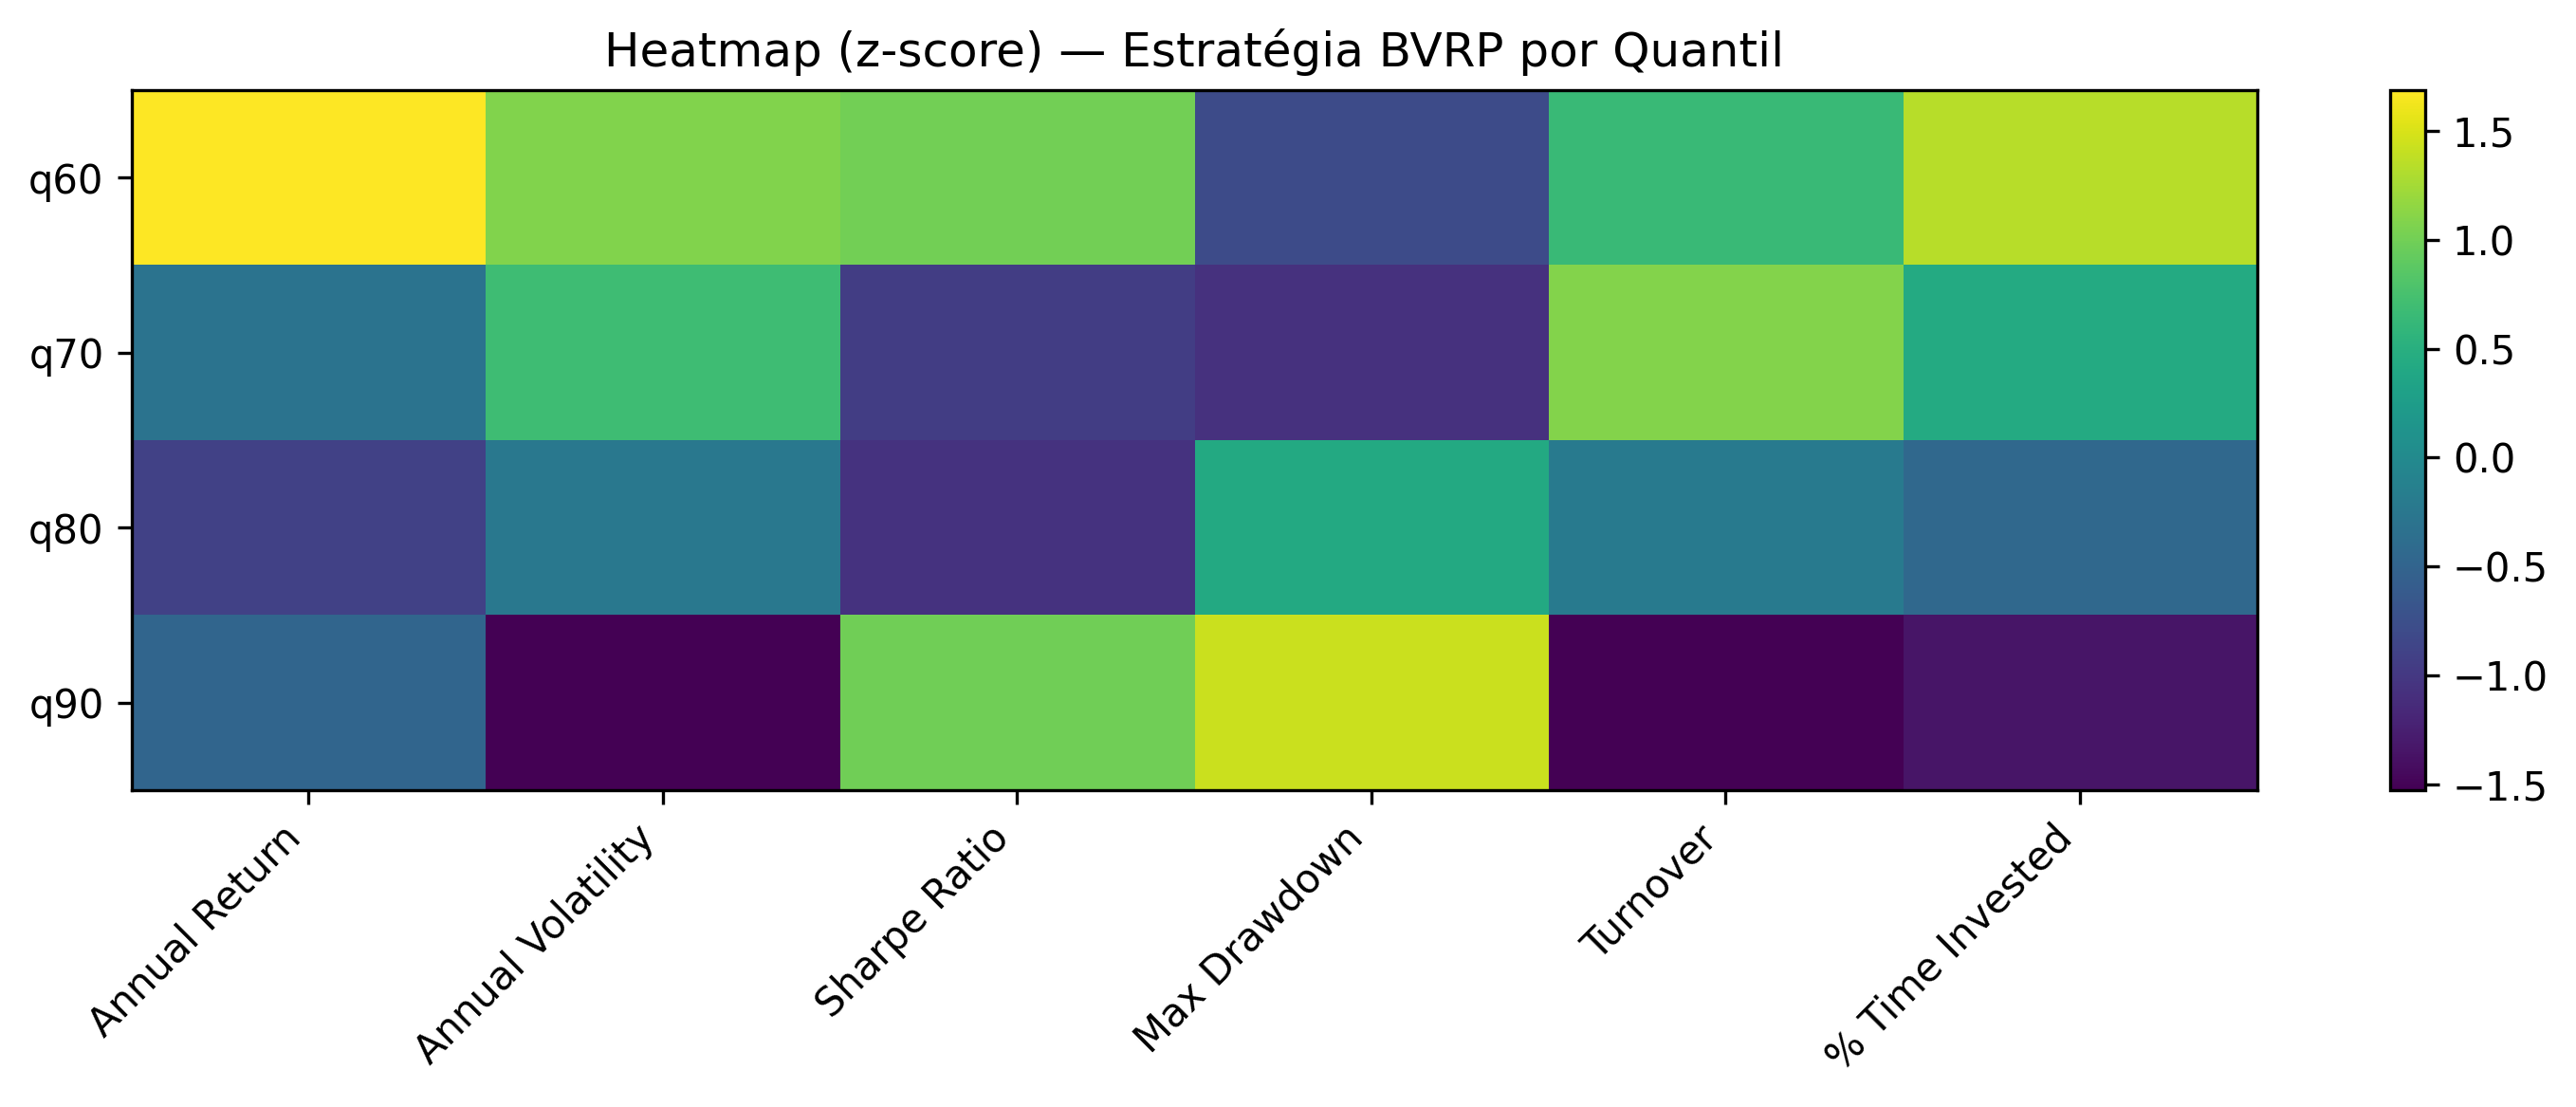
\includegraphics[width=0.97\textwidth]{figs/cap7/fig_7_03_heatmap_bvrp_quantile_metrics.png}
\caption{Heatmap (z-score) — Sensibilidade das métricas de desempenho e operação aos quantis do BVRP}
\label{fig:cap7_bvrp_heatmap}
\end{figure}

Sob a ótica econômica, a variação das métricas ao longo dos quantis sugere que o
BVRP contém informação condicional relevante sobre o trade-off intertemporal
entre retorno esperado e risco. Quantis mais elevados tendem a coincidir com
estados de maior aversão ao risco e/ou incerteza elevada, nos quais o prêmio
exigido para carregar risco de volatilidade é maior.

À luz dos resultados, o quantil de 80\% do BVRP é adotado como especificação de
referência nas análises subsequentes, por representar um compromisso entre
seletividade do sinal, estabilidade do desempenho ajustado ao risco e intensidade
operacional. Esse limiar reduz a diluição informacional de quantis muito baixos
e evita dependência excessiva de poucos eventos extremos, mais típica de quantis
muito elevados.

% =========================================================
\section{Estratégias Condicionais ao BVRP por Regime de Volatilidade}
\label{sec:cap7_bvrp_regimes}

Esta seção investiga a interação entre o BVRP e regimes de volatilidade realizada,
avaliando se a eficácia do sinal depende do ambiente de risco prevalente no mercado.
Os regimes são definidos a partir dos tercis da distribuição da volatilidade realizada
de 30 dias ($RV_{30}$), classificando os dias em baixa, média e alta volatilidade.

Mantém-se a regra condicional ao BVRP (quantil de 80\%), mas restringe-se a tomada
de posição aos dias pertencentes a cada regime específico. Em termos práticos, a
estratégia opera apenas dentro do subconjunto de datas do regime; fora dele, a
posição é neutra. O objetivo é isolar estados do mundo em que o BVRP pode ser mais
(ou menos) informativo, distinguindo entre ambientes calmos e ambientes de estresse.

A Tabela~\ref{tab:cap7_bvrp_regimes_perf} reporta as métricas de desempenho e as
estatísticas operacionais por regime, enquanto a Figura~\ref{fig:cap7_bvrp_regimes_cumret}
apresenta a evolução do retorno acumulado correspondente.

\begin{table}[H]
\centering
\caption{Desempenho da estratégia BVRP (quantil 80\%) por regime de volatilidade}
\label{tab:cap7_bvrp_regimes_perf}
\resizebox{\textwidth}{!}{%
\begin{tabular}{lrrrrrr}
\toprule
 & Retorno Anual & Volatilidade Anual & Sharpe Ratio & Max Drawdown & Turnover & \% Tempo Investido \\
Regime de RV &  &  &  &  &  &  \\
\midrule
Baixa RV & 0.0231 & 0.1360 & 0.1699 & -0.1469 & 0.0289 & 0.1124 \\
Media RV & 0.2195 & 0.1729 & 1.2693 & -0.1272 & 0.0386 & 0.0674 \\
Alta RV & -0.0162 & 0.0939 & -0.1725 & -0.1087 & 0.0096 & 0.0209 \\
\bottomrule
\end{tabular}
}
\end{table}

\begin{figure}[H]
\centering
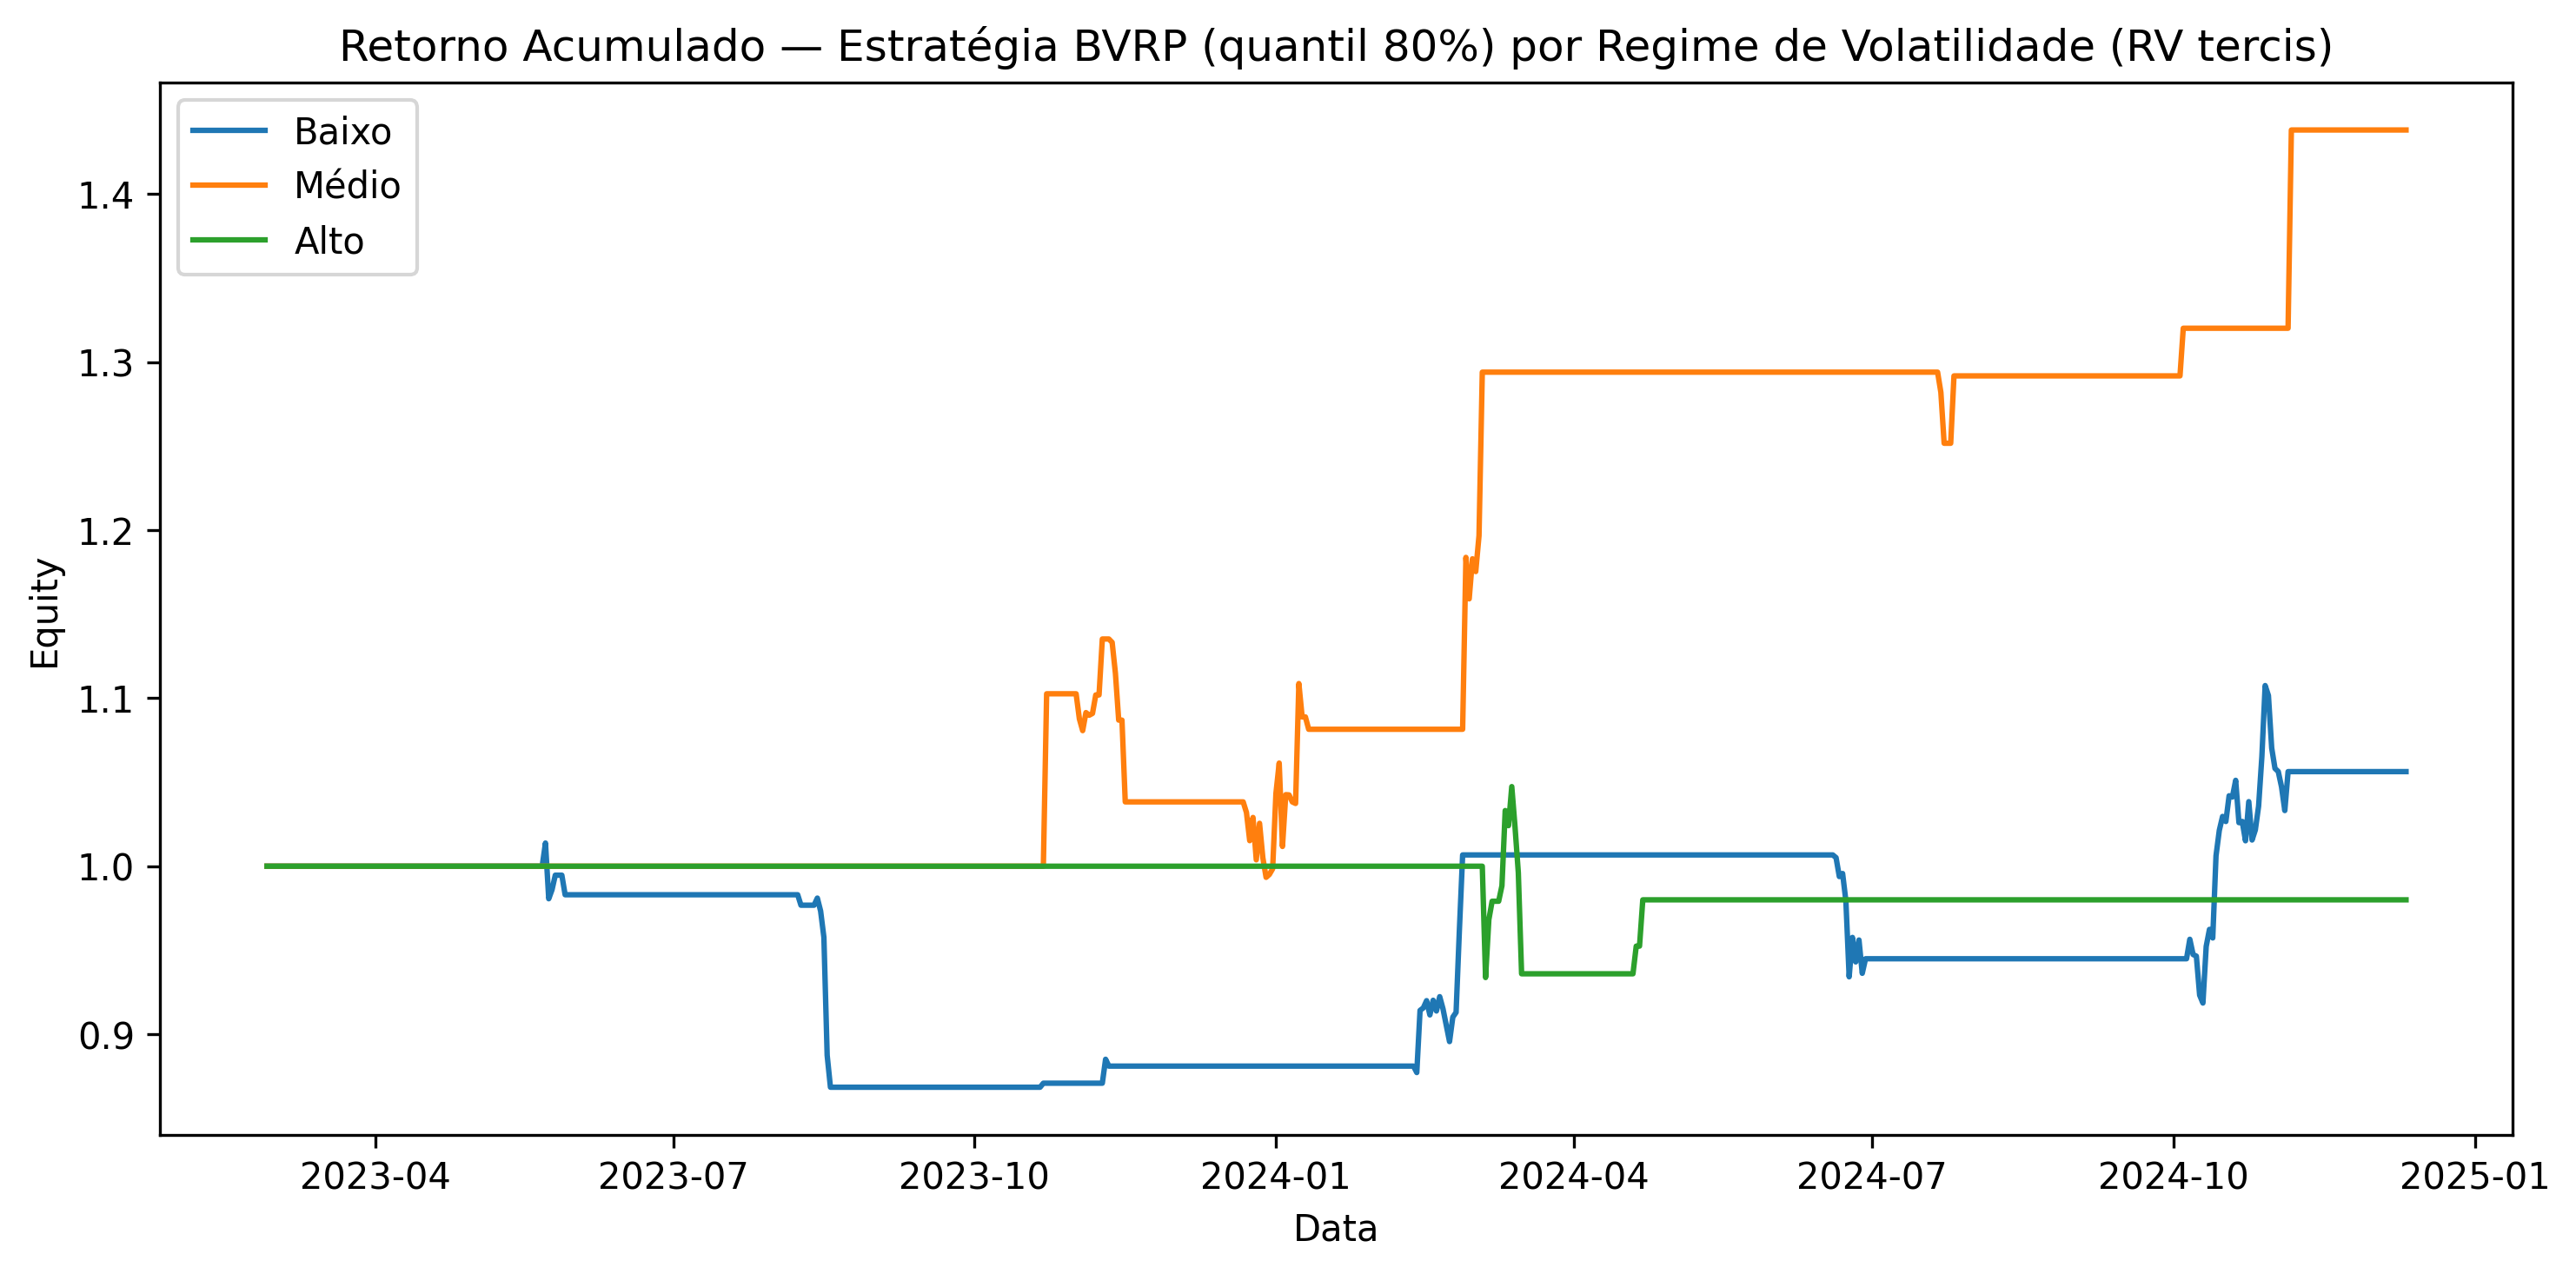
\includegraphics[width=0.95\textwidth]{figs/cap7/fig_7_04_cum_returns_bvrp_by_regime.png}
\caption{Retorno acumulado da estratégia BVRP (quantil 80\%) por regime de volatilidade}
\label{fig:cap7_bvrp_regimes_cumret}
\end{figure}

Os resultados indicam que a eficácia do BVRP como sinal de negociação depende do
regime de volatilidade realizada. Em particular, o desempenho ajustado ao risco tende
a ser superior em períodos de alta volatilidade, nos quais o prêmio exigido pelos
investidores para assumir risco de volatilidade é maior e o mercado apresenta maior
heterogeneidade de crenças e demanda por proteção.

Esse comportamento é consistente com a interpretação do BVRP como uma medida
condicional de aversão ao risco e de precificação de incerteza, cuja capacidade
informacional se intensifica em ambientes de maior estresse. Em regimes de baixa
volatilidade, o sinal tende a ser menos discriminatório, reduzindo a diferença de
desempenho em relação ao \textit{benchmark} e aumentando a probabilidade de que o
ganho observado reflita ruído amostral.

% =========================================================
\section{Síntese Empírica e Implicações}
\label{sec:cap7_sintese}

As análises empíricas desenvolvidas ao longo deste capítulo fornecem evidências de
que o Prêmio de Risco de Volatilidade do Bitcoin (BVRP) pode ser explorado como
sinal para estratégias condicionais, produzindo perfis de retorno e risco distintos
da estratégia passiva de Buy-and-Hold, frequentemente com menor tempo de exposição
ao ativo e redução de perdas extremas.

A estratégia condicional baseada no quantil superior do BVRP
(Seção~\ref{sec:cap7_bvrp_q}) sugere que períodos de prêmio elevado tendem a estar
associados a janelas com melhor compensação pelo risco assumido, resultando em
métricas ajustadas ao risco favoráveis em comparação ao \textit{benchmark}, ainda
que com participação intermitente no mercado. A análise de robustez por quantis
(Seção~\ref{sec:cap7_bvrp_multiq}) indica que o desempenho depende do grau de
seletividade: limiares muito baixos diluem o sinal, enquanto limiares muito altos
concentram a estratégia em poucos episódios, elevando a variância amostral.

A extensão por regimes de volatilidade realizada
(Seção~\ref{sec:cap7_bvrp_regimes}) mostra que a utilidade do BVRP é dependente do
estado do mercado. Em ambientes de alta volatilidade, o sinal tende a ser mais
discriminatório, ao passo que em ambientes de baixa volatilidade a evidência é
mais fraca. Em conjunto, esses resultados são coerentes com a interpretação do
BVRP como prêmio associado à aversão ao risco e à demanda por proteção, mais
relevante em períodos de estresse.

Por fim, as estratégias analisadas utilizam regras com limiares fixos e uma única
variável de sinal, o que limita a capacidade de capturar interações dinâmicas com
outras variáveis de mercado e potenciais não linearidades. Essas limitações motivam
a consideração de extensões orientadas a dados e de modelos mais flexíveis, bem como
a avaliação cuidadosa de custos de transação, fricções e restrições operacionais,
de modo a aproximar os resultados de um ambiente de implementação realista.
